\chapter{相关工作 }\label{chap:related_work}
% 2.1边缘计算技术,多终端,协同,服务
%     2.2docker容器技术/容器集群技术
%     2.3自组织网络技术——对应研究点1
%     2.4启发式调度算法——对应研究点2  可能会换成任务调度算法
%     2.5计算迁移——对应研究点3
%     2.6预测算法——对应研究点4

\section{引言}
% 这里再加上几个点的关系,先是介绍终端协同服务技术,然后说对资源的利用,虚拟化技术,然后说计算迁移技术,最后说任务调度
本文主要研究解决终端资源利用和终端服务优化问题的基于容器化多终端协同服务技术。本章对于本文的研究所涉及到的相关背景和相关技术进行铺垫和介绍,为后续章节对本文的研究内容进行详细介绍打下基础。

本章的内容结构组织如下:第\ref{sec:related_work_cloud_computing}节介绍云计算技术与边缘计算技术的相关概念和特点;第\ref{sec:related_work_virtualization}节介绍了虚拟化技术特别是容器虚拟化技术的发展现状;第\ref{sec:related_work_computing_offloading}节介绍了计算迁移技术的研究现状;第\ref{sec:related_work_task_scheduling}节介绍了任务调度问题及元启发式算法的研究进展;第\ref{sec:related_work_summary}节总结了本章内容。

\section{终端协同服务技术}\label{sec:related_work_cloud_computing}
% 这里可以加一下,介绍终端协同服务的概念以及跟其他几个资源利用技术的关系
随着信息技术的快速发展,应用和服务对于计算、存储等资源的需求也越来越高,单一计算设备所能提供的计算、存储资源难以满足这些服务对于硬件计算、存储能力的需求。为了解决这一问题,越来越多的计算模式被研究人员所提出。云计算技术主要利用云数据中心近乎无限的资源为远端用户提供服务。随着物联网、大数据等技术的快速发展,传统的云计算模式存在实时性、安全性等问题,因此进行计算的位置逐渐由云端数据中心逐渐向网络边缘转移,出现了雾计算、边缘计算、海服务等计算模式。
% 随着移动网络的高速发展,5G时代即将到来,移动云计算慢慢兴起。
本研究所关注的终端协同服务技术是一种利用多个智能终端上的计算、存储等资源协同合作为用户提供服务的技术。终端协同服务技术主要关注网络边缘小范围内多个智能终端之间的资源利用与服务质量保证的问题,是一种自下而上的计算模式。虽然应用层次不同,但是传统的云计算、边缘计算等计算模式能够为终端协同服务技术提供很多经验。

\subsection{云计算技术}
% //TODO:增加一个云计算的架构图
随着处理和存储技术的快速发展以及互联网的普及,计算资源变得比以往任何时候都更便宜,更强大,更普遍。这种技术趋势使得云计算的计算模型成为现实。云计算是一种通过互联网管理和提供服务的范例\cite{zhang2010cloud,josep2010view}。云计算的思想很早之前就存在,20世纪60年代,约翰·麦卡锡已经设想计算设施将像一种工具(Unity)一样提供给公众\cite{parkhill1966challenge}。但是直到2006年谷歌公司(Google)使用“云计算”一词来描述通过网络提供服务的商业模型,云计算的概念才开始流行起来。云计算的概念虽然已经发展了很多年,但是并没有一个标准的定义\cite{sonnek2009virtual},这里采用美国国家标准技术研究院(The National Institute of Standards and Technology,NIST)给出的定义\cite{zhang2010cloud}:云计算是一种可以方便地通过网络来按需对可配置的共享计算资源池(如网络、服务器、存储、应用和服务等)进行访问的模型,可以以最少的管理工作或与服务提供商交互的方式来进行快速配置和发布。

云计算可以根据服务模式不同,划分为基础设施即是服务(Infrastructure as a Service,IaaS),平台即是服务(Platform as a Service,PaaS),软件即是服务(Software as a Service,SaaS)\cite{林伟伟2012云计算资源调度研究综述,roman2018mobile}。云计算中的三种服务模式结构如图\ref{fig:cloud_computation_S_P_I}所示\cite{刘英男2011基于云计算框架的终端管理系统设计与实现}。

\begin{figure}[!htbp]
    \centering
    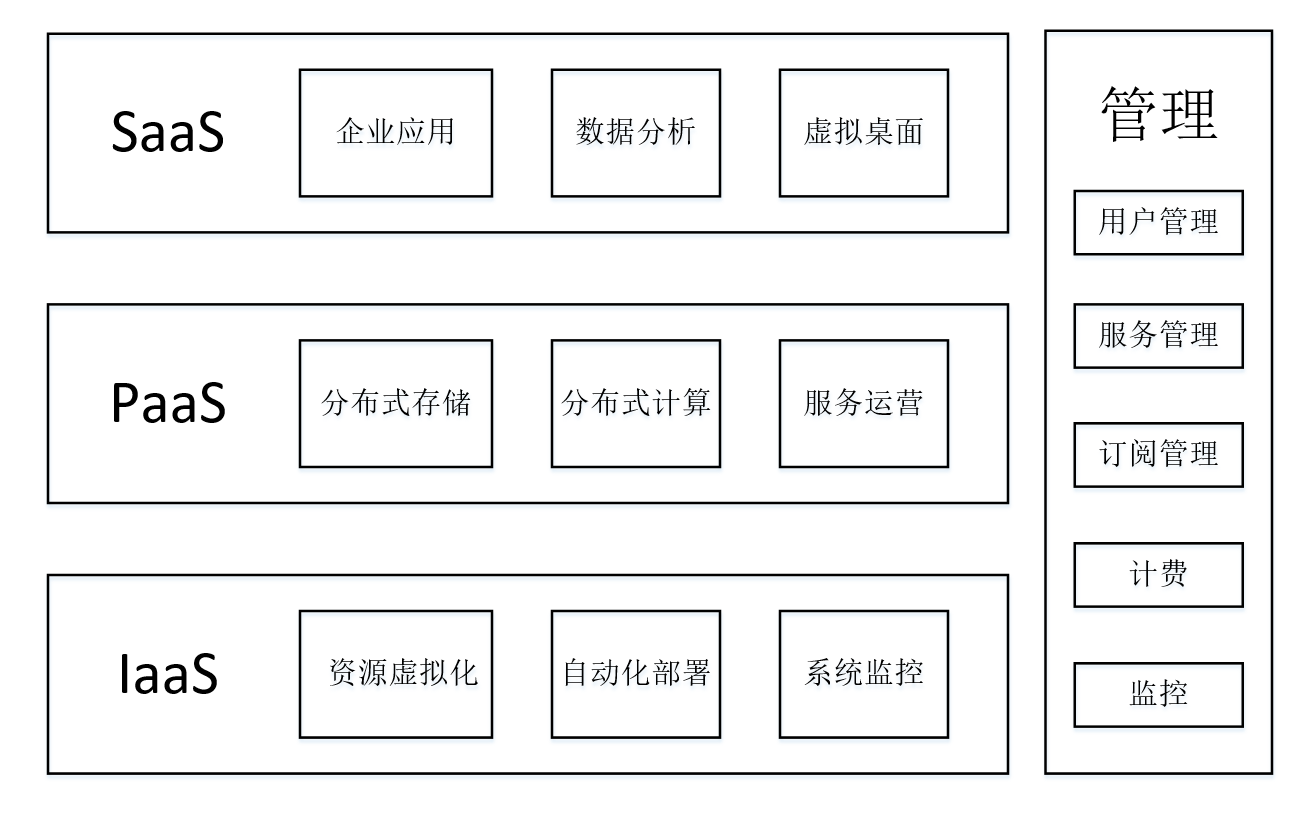
\includegraphics[width=1.0\textwidth]{Cloud_Computation_S_P_I_Temp}
    \caption{云计算种三种服务模式结构图}
    \label{fig:cloud_computation_S_P_I}
\end{figure}

IaaS是运行云所需的承载、硬件配置和基本服务的组合,使用虚拟化技术将基础设施层的硬件资源如计算、存储等,封装起来并对外提供。
PaaS平台的主要指的是云服务提供商为企业提供的计算平台以及相关软件应用程序集(解决方案堆栈)的提供和部署。
SaaS是一种软件分发模型,这种模型中,应用程序由供应商或服务提供商托管并通过网络向客户提供\cite{manvi2014resource}。

云计算还拥有以下特点:云计算可根据需要提供无限计算资源,从而消除了云计算用户对供应计划的需求;云计算可以消除云用户的提前计划配置要求,从而允许公司从小规模开始做起,只有在需求增加时才增加硬件资源,这对企业用户来说也很有吸引力;云计算拥有根据需要支付短期使用的计算资源的能力(例如,按小时计算的处理器资源和按天计算的存储资源),并根据需要释放它们\cite{fox2009above}。

\subsection{雾计算技术}

在云计算中,用户设备的信息数据需要发送到集中式的云数据中心进行处理,长距离的信息传输会产生较高的响应时延,这会造成一些要求快速响应的服务质量较差。另外云计算模式中用户设备与远端的云数据中心进行数据交互,也会产生隐私泄露、用户信息被窃取等安全性问题。

为了解决云计算中存在的这些问题,研究人员将能够提供计算和存储能力的设备部署在终端与云端之间,拉近用户终端与计算资源之间的距离,这样就产生了雾计算(Fog Computing)的概念。雾计算最早是由思科(Cisco)提出的一种计算模式。雾计算在云端数据中心与网络边缘终端之间引入雾层的概念,在雾层部署独立的计算、通信、存储、控制设备,在比云端数据中心更靠近用户的地方为用户提供服务\cite{贾维嘉2018雾计算的概念}。
% //TODO:增加一个云计算的架构图

雾计算的架构图如图所示。从思科对雾计算的定义与解释来看,雾计算被认为是云计算模式从网络核心到网络边缘的一种扩展范式。在思科提出的雾计算思想基础上,HP实验室对雾计算给出了更进一步的定义:“一种大量异构的、普遍分布的、去中心化分布设备(通过无线网络进行连接,有的时候是自治的)互相通信互相协作并且在没有第三方干扰的情况下通过网络提供存储服务和执行计算任务的场景”\cite{vaquero2014finding}。IOx是思科提供的雾设备产品,通过在连接网格路由器(Connected Grid Router, CGR)上直接运行在虚拟机管理程序(Hypervisior)上的客户操作系统(Guest Operating System, GOS)中托管应用程序来进行工作\cite{yi2015survey},用户可以利用IOx框架来将自己开发的应用部署到雾计算支持的设备节点上。2015年11月,ARM、思科、戴尔(Dell)、英特尔(Intel)、微软(Microsoft)和美国普林斯顿大学联合成立了开放雾联盟(Open Fog Consortium)该联盟旨在通过开发开放式架构、分布式计算、联网和存储等核心技术以及实现物联网全部潜力所需的领导力,加快雾计算的部署\cite{李子姝2018移动边缘计算综述}。

雾计算可以被认为是云计算的一种补充,但是在访问方式、控制管理、服务质量、采用设备、目标用户等方面与云计算还存在着很多不同之处,文献\cite{贾维嘉2018雾计算的概念}对此进行了比较和总结,总结结果如表\ref{tab:compare_fog_cloud}所示。

\begin{table}[!htbp]
    \centering
    \caption{雾计算和云计算的比较}\label{tab:compare_fog_cloud}
    \renewcommand\arraystretch{1.0} 
    \scriptsize
    % \small
\begin{tabular}{*{4}{l}}
    \hline
    方面 & 具体指标& 云计算 & 雾计算\\
    \hline
    \multirow{6}*{通信访问方式}
    & 节点的访问方式& 通过互联网& 通过本地网络设施\\
    & 服务的访问方式& 通过核心网& 通过边缘设备\\
    & 终端用户到节点距离& 多跳& 一跳\\
    & 对于移动前传和集中式的基带单元的负担& 重& 轻\\
    & 缓存与无线信号处理& 集中式& 兼具集中式与分布式\\
    & 无限资源管理& 集中式& 兼具集中式与分布式\\
    \hline
    \multirow{11}*{服务质量}
    & 时延& 较高(分钟级~月级)& 较低(毫秒级~秒级)\\
    & 时延抖动& 高& 很低\\
    & 可用性& 99.99\% & 不定\\
    & 数据传输过程受攻击可能性& 可能性高& 可能性很低\\
    & 安全策略& 难以定义& 易被定义\\
    & 移动性支持& 有限支持& 支持程度高\\
    & 服务来源& 全球& 本地\\
    & 使用成本& 高& 低\\
    & 网络要求& 高& 低    \\
    & 对实时应用的支持& 差& 好\\
    & 任务的传输功耗& 大& 小\\
    \hline
    \multirow{8}*{服务质量}
    & 终端用户数& 数十万或数百万& 数十万\\
    & 节点数目& 少& 多\\
    & 硬件设备平均成本/美元& 1 500~3 000& 50~200\\
    & 设备部署位置& 远端数据中心& 靠近网络边缘\\
    & 硬件& 存储容量大、计算能力强& 存储容量与计算能力有限    \\
    & 设备部署环境& 带制冷设备的大型仓库& 小型仓库或室外\\
    & 服务器拥有者与管理者& 大公司(如 Google)& 小公司或个人\\
    & 部署速度(代价)& 慢& 快\\
    \hline
    \multirow{6}*{通信访问方式}
    & 节点的访问方式& 通过互联网& 通过本地网络设施\\
    & 服务的访问方式& 通过核心网& 通过边缘设备\\
    & 终端用户到节点距离& 多跳& 一跳\\
    & 对于移动前传和集中式的基带单元的负担& 重& 轻\\
    & 缓存与无线信号处理& 集中式& 兼具集中式与分布式\\
    & 无限资源管理& 集中式& 兼具集中式与分布式\\
    \hline
    \multirow{3}*{通信访问方式}
    & 内容产生者& 主要是人& 主要是传感器设备\\
    & 内容丰富程度& 丰富& 单一\\
    & 目标用户& 互联网用户& 移动用户\\
    \hline
   \end{tabular}
\end{table}

雾计算拥有很多应用场景。

\subsection{边缘计算技术}
% 这里可能还要加一些物联网、智慧城市、移动边缘计算、cloudlet等方面的研究内容,以及边缘计算的应用场景
% 再加上一些微信分享内容

相比雾计算,边缘计算(Edge Computing)将计算资源推向离用户更近的网络边缘。这里采用文献\cite{施巍松2017边缘计算}中提出的边缘计算的定义:“边缘计算是指在网络边缘执行计算的一种新型计算模式,边缘计算中边缘的下行数据表示云服务,上行数据表示万物互联服务,而边缘计算的边缘是指从数据源到云计算中心路径之间的任意计算和网络资源”。根据这个定义,边缘计算的模式如图\ref{fig:edge_computing_paradigm}所示\cite{shi2016edge}。

\begin{figure}[!htbp]
    \centering
    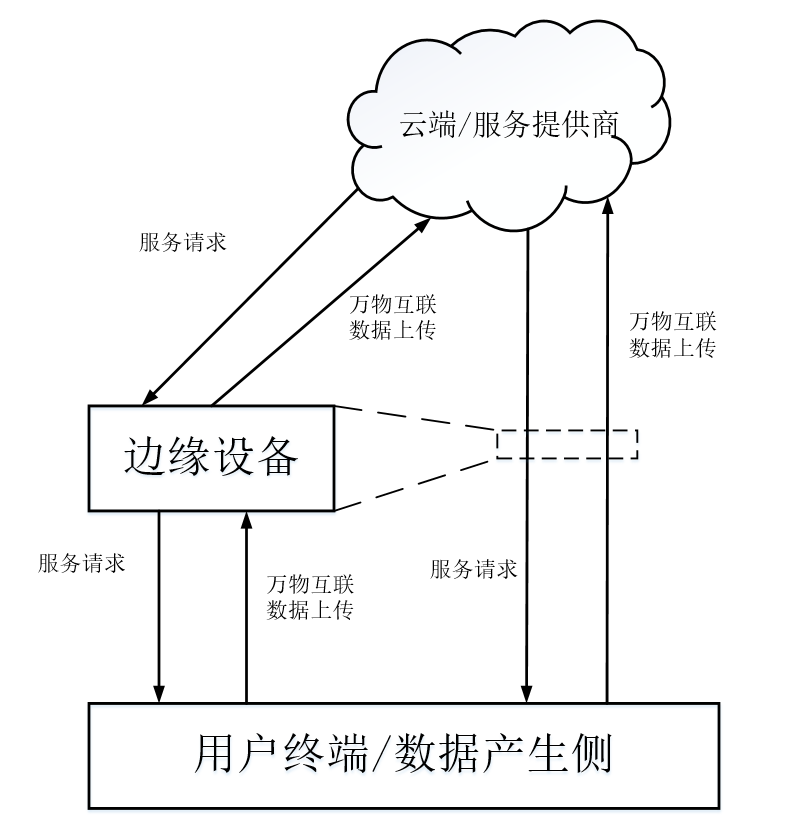
\includegraphics[width=1.0\textwidth]{Edge_Computing_Paradigm_Temp}
    \caption{边缘计算模式结构图}
    \label{fig:edge_computing_paradigm}
\end{figure}

在边缘计算范例中,边缘终端设备不仅是数据消费者,而且还充当数据产生者。在边缘终端上不仅可以从云端请求服务和数据,还可以作为云端来执行计算任务。边缘侧可以执行计算迁移,数据存储,缓存和处理,以及从云向用户分发请求和交付服务\cite{shi2016edge}。

相比云计算,边缘计算拥有很多优点\cite{赵梓铭2018边缘计算}。利用边缘设备上的计算能力可以执行很多用户终端的计算任务,可以为云端数据中心分担计算压力,而且基于边缘设备对一些用户上传数据的预处理,可以抛弃大量冗余数据,精简压缩上行数据包,缓解网络带宽压力。边缘设备距离用户侧也更近,一些原本需要到云端去执行的任务可以放到边缘设备上来进行计算,减少传输延迟,缩短服务响应时间,提高用户体验。另外,由于在边缘计算的模式中,数据可以在边缘设备上进行处理,而不用将被上传到远程云数据中心,这就减少了隐私数据传输过程总被窃取以及在云端被第三方盗用的风险,提高了用户隐私数据的安全性。严格意义上来讲,本文所研究的多终端协同服务技术,也属于边缘计算中的一种场景。
% 边缘计算的应用场景包括:。


% \subsection{移动云计算}

\subsection{海服务}

\subsection{终端协同服务技术}



\section{虚拟化技术}\label{sec:related_work_virtualization}
资源管理问题是协同服务技术中的一个重要的问题\citep{文雨2013面向应用服务级目标的虚拟化资源管理}。而虚拟化技术是解决资源管理问题的一个重要的解决办法。虚拟化技术是一种资源管理技术,利用底层虚拟、上层隔离等方法,将计算机中的物理资源,如计算、存储和网络等,进行抽象、切割,以更好的形式提供给用户使用\cite{goth2007virtualization}。虚拟化技术将计算机上原有的固定配额的物理资源按照用户需要很方便地进行分配、提取和利用,可以提高计算机和终端资源的利用率。

1959年,克里斯托弗(Christopher Strachey)在他的学术报告《大型高速计算机中的时间共享》中提出了虚拟化的基本概念,成为了虚拟化技术的开端\citep{本刊编辑部2017虚拟化概述}。虽然随着计算机技术的发展,硬件价格的下降与用户需求的变化使得虚拟化技术的研究与应用一度陷入低谷,但是随着云计算等概念的兴起以及互联网服务模式的革命性变化,虚拟化技术又重新成为学术界和工业界研究的热点\cite{menasce2005virtualization}。在IBM公司、HP公司、VMWare公司等企业的不断努力下,经过了60年的发展和成熟,虚拟化技术逐渐成为云计算与边缘计算中非常重要的一种资源管理技术\cite{pearce2013virtualization,kumar2014review}。

用户根据自己的需求来租赁云计算或边缘计算的服务提供商所提供的对应资源配额的虚拟机,直接在虚拟化的操作系统中运行用户自己的应用而不需要考虑操作系统底层是如何实现的,就如同运行在一个真实而独立的实体物理机一样,非常透明\cite{叶蔚2019基于虚拟化的}。而虚拟化技术则被用来实现虚拟机的生命周期管理,包括创建、配置、关闭、监控、释放资源等等,维持这种对用户的透明性。服务提供商利用虚拟化技术,以虚拟机的形式为用户提供服务,可以让一台服务器同时支持多个用户独立访问,且每个用户之间是完全独立的,提高了服务提供商的资源利用率,降低了云服务提供的成本,同时虚拟机互相隔离的特性也提升了云服务的安全性。

虚拟化技术为云计算技术打下了良好的基础。应用了虚拟化技术的云计算模型如图\ref{fig:cloud_computation_virtualization}所示\citep{陈思锦2015云计算中的虚拟化技术与虚拟化安全}。第\ref{sec:related_work_cloud_computing}节中提到,云计算中所能够提供的服务包括基础设施即是服务(IaaS)、平台即是服务(PaaS)和软件即是服务(SaaS),这三种服务模式都离不开虚拟化技术的支持。IaaS能够为用户提供计算、存储等资源,这些都需要利用虚拟化技术来进行资源的抽象、资源数量的划分,并且封装成虚拟机来提供给用户远程使用。在用户使用这些资源的过程中,也要受到虚拟化技术对资源使用数量和时间的监控和管理,以及对虚拟机生命周期的管理。PaaS能够为用户提供计算平台、相关软件应用程序集以及应用部署的平台。PaaS除了利用虚拟化技术对资源进行管理,还利用了虚拟化技术的封装的特性,将提前封装好的包含相关软件应用程序集的应用运行环境提供给用户,并且以虚拟机为单位进行部署和运维。SaaS在以上两种服务的基础上,利用了虚拟化技术的隔离和透明的特性,将应用程序封装在虚拟机中,通过网络向用户提供服务,用户不必关心应用本身是运行在虚拟机中还是独立的物理服务器中。这些虚拟机彼此之间是隔离的,一台服务器可以同时运行多个虚拟机独立为用户提供服务,同一台服务器上的不同虚拟机之间不会互通,保证了服务的安全性。另外,虚拟化技术在面对云计算中的分布式计算、权限管理、服务器灾难恢复等问题以及在为科学计算中的网络、安全等领域提供实验环境方面也能够提供比较合适的解决方案\cite{2008半虚拟化技术分析与研究}。


\begin{figure}[!htbp]
    \centering
    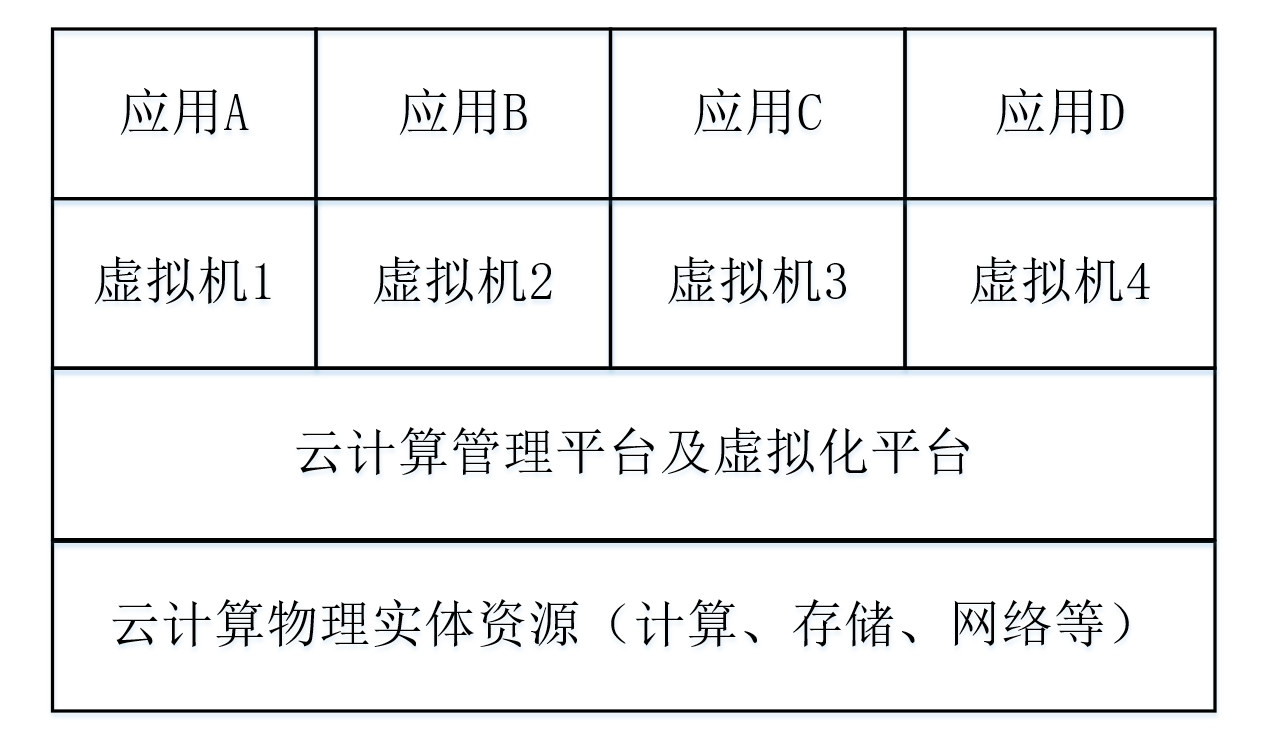
\includegraphics[width=1.0\textwidth]{Cloud_Computation_Virtualization_Temp}
    \caption{应用了虚拟化技术的云计算模型}
    \label{fig:cloud_computation_virtualization}
\end{figure}

虚拟化技术自1959年被提出,经历了硬件分区技术、完全虚拟化技术、半虚拟化技术和操作系统虚拟化技术等几个发展阶段\cite{肖伟民2019嵌入式虚拟化},从底层硬件层逐渐向操作系统层过渡,逐渐成为一种成熟的资源管理技术。

\subsection{硬件分区技术}

硬件分区技术是早期的虚拟化技术。硬件资源被划分为互相独立的分区,每个分区的存储和计算资源是独立的,也会安装独立的操作系统\cite{plessl2004virtualization}。硬件分区技术可以做到对资源进行比较细粒度的划分,但这种划分比较简单,不够灵活,也不方便系统对资源进行管理。硬件分区技术的架构图如图\ref{fig:hardware_virtualization}所示\cite{肖伟民2019嵌入式虚拟化}。

\begin{figure}[!htbp]
    \centering
    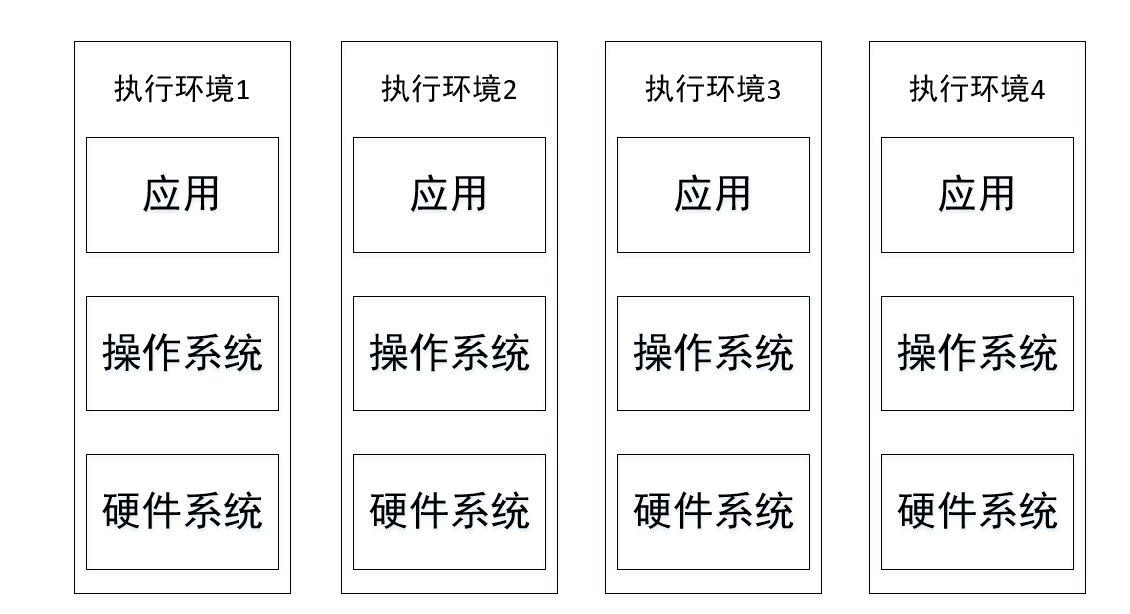
\includegraphics[width=1.0\textwidth]{Hardware_Virtualization_Temp}
    \caption{硬件分区技术架构}
    \label{fig:hardware_virtualization}
\end{figure}

\subsection{完全虚拟化技术}

完全虚拟化技术(Full Virtualization Technology)通过在宿主机操作系统(Host Operation System, Host OS)上面架设一层虚拟机监控器(Virtual Machine Monitor, VMM)\citep{li2017performance}来实现对硬件的虚拟化,完全虚拟化技术中的虚拟机监控器,通常为超级监控器,即Hypervisor或者Supervisor\citep{kolhe2012comparative}\citep{leite2012performance}。VMM在虚拟硬件的基础上再进一步虚拟出一套用户的操作系统(Guest Operation System, Guest OS),供用户操作使用。为了方便阐述,在本文中,通过完全虚拟化技术实现的虚拟机简称为VM虚拟机。完全虚拟化技术的架构如图\ref{fig:full_virtualization}所示\citep{oludele2014evolution}。

\begin{figure}[!htbp]
    \centering
    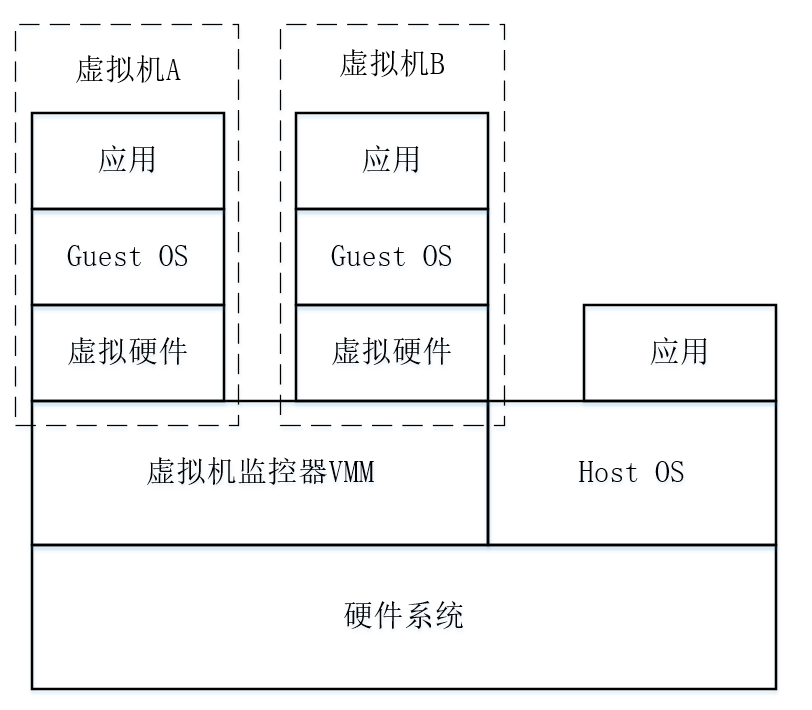
\includegraphics[width=1.0\textwidth]{Full_Virtualization_Temp}
    \caption{完全虚拟化技术架构}
    \label{fig:full_virtualization}
\end{figure}

云计算行业内曾经非常流行的工具如VMware\citep{sahasrabudhe2014comparing,li2010selecting}、KVM\citep{liu2014research}、VirtualBox\citep{li2010selecting}等,都属于比较传统的完全虚拟化技术,这些完全虚拟化工具都拥有非常良好的对硬件资源的管理、隔离、虚拟、利用的功能。但是另一方面,完全虚拟化技术使用了虚拟机监控器VMM来虚拟硬件层,能够提供相对较完整独立、隔离性好的虚拟化环境,但是启动速度慢,需要消耗大量额外资源来维持虚拟化环境。

\subsection{半虚拟化技术}

半虚拟化技术(Para-Virtualization)是由完全虚拟化技术发展而来的。为了改善完全虚拟化技术的性能,半虚拟技术对客户操作系统内核做了一些优化,将一些底层CPU执行的任务转移到操作系统内核中完成。半虚拟化技术的架构图如图\ref{fig:para_virtualization}所示\cite{2008半虚拟化技术分析与研究}。

\begin{figure}[!htbp]
    \centering
    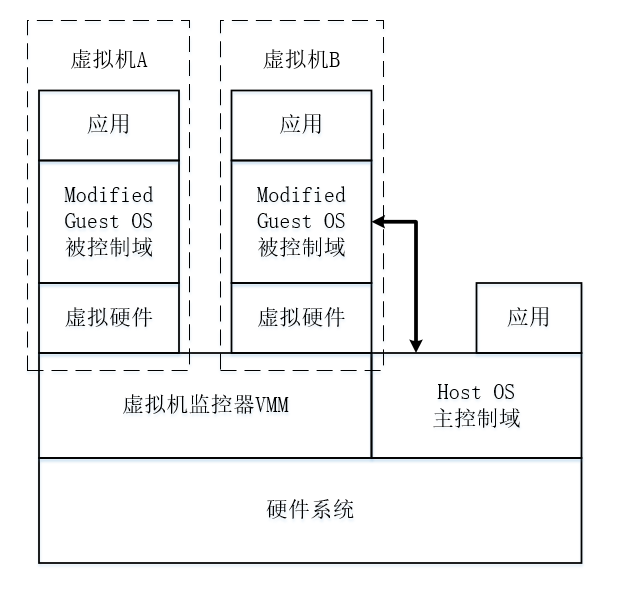
\includegraphics[width=1.0\textwidth]{Para_Virtualization_Temp}
    \caption{半虚拟化技术架构}
    \label{fig:para_virtualization}
\end{figure}

半虚拟化技术的代表是Xen\cite{barham2003xen}。半虚拟化技术比完全虚拟化技术性能好,但是需要对操作系统内核进行修改。

\subsection{操作系统级虚拟化技术}

操作系统级虚拟化技术(Operation System Virtualization Technology),是一种轻量级虚拟化技术\citep{morabito2017virtualization}。与传统的完全虚拟化技术相比,操作系统级虚拟化技术不需要对底层硬件进行虚拟化,而是直接在操作系统层上采用隔离的方法虚拟出与宿主机操作系统互相隔离的虚拟机。对此有一个生动形象的比喻,如果将物理实体宿主机比作一座房子,那么其底层硬件则是地基,操作系统是房子的支撑墙,系统中运行的应用则是房子内的具体房间。而传统的完全虚拟化技术可以比喻为在原有房子的地基之上另外实现一层新的地基(虚拟机监控器VMM),并在新地基上重新修建支撑墙(Guest OS)和房间(虚拟机)。相应地,操作系统级虚拟化技术则是直接借用了宿主机原有的地基(底层硬件)和支撑墙(操作系统),并在原来的房间里利用隔板隔离出来新的房间(虚拟机)。操作系统级虚拟化技术的架构如图\ref{fig:os_virtualization}所示\citep{xavier2013performance}。由于没有使用虚拟机监控器VMM来对硬件进行虚拟化,所以操作系统级虚拟化技术启动速度非常快,而且也不会消耗非常多的额外虚拟化开销,非常轻量级\citep{babu2014system}。

\begin{figure}[!htbp]
    \centering
    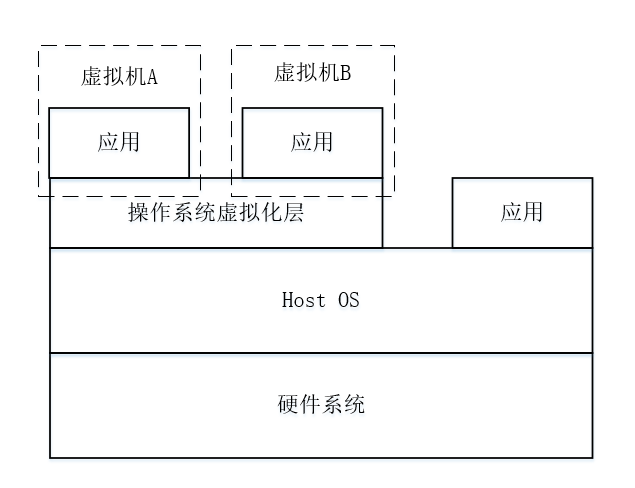
\includegraphics[width=1.0\textwidth]{OS_Virtualization_Temp}
    \caption{操作系统级虚拟化技术架构}
    \label{fig:os_virtualization}
\end{figure}

\subsection{容器虚拟化技术}

容器虚拟化技术(Container Virtualization Technology)属于操作系统级虚拟化技术的一种\citep{vaughan2006new}。容器虚拟化技术虚拟出来的“虚拟机”通常被称为容器(Container)。容器技术底层使用的是基于Linux内核的Linux Container(LXC)技术,而不需要进行额外的虚拟化操作\cite{celesti2016exploring}。LXC技术的核心技术包括Namespace技术和Cgroups技术\cite{肖伟民2019嵌入式虚拟化}。Namespace技术可以为容器提供一个独立的、隔离的命名空间,其中包含PID(进程)、UTS(host name)、MNT(文件)、NET(网络)、IPC(进程间交互)、USER(用户)等六个方面\cite{liu2014researchandimplementation}。六种namespace隔离的系统调用如表\ref{tab:namespace_system}所示。

\begin{table}[!htbp]
    \centering
    \caption{namespace隔离的六个方面}\label{tab:namespace_system}
    \renewcommand\arraystretch{1.5} 
    % \scriptsize
\begin{tabular}{*{3}{c}}
    \hline
    Namespace & 系统调用参数& 隔离内容\\
    \hline
    UTS & CLONE\_NEWUTS & 主机名与域名 \\
    IPC	& CLONE\_NEWIPC & 信号量、消息队列和共享内存\\
    PID & CLONE\_NEWPID & 进程编号\\
    Network & CLONE\_NEWNET & 网络设备、网络栈、端口等等 \\
    Mount & CLONE\_NEWNS & 挂载点(文件系统)\\
    User & CLONE\_NEWUSER & 用户和用户组\\
    \hline
   \end{tabular}
\end{table}

不同命名空间的进程彼此之间看不到,Namespace单独隔离出来的命名空间中的容器与其宿主机之间也是彼此看不到,只能通过UTS将对方当作网络中的另一个主机节点,这样就保持了容器的独立性和隔离性。而通过Cgroups技术,可以对每个容器所拥有的CPU、内存、存储、输入输出等资源进行进程级别的管理和配置,这样就使得用户可以利用容器对终端资源进行按需分配管理。同时,利用Cgroups控制组,也能够对对容器内各种资源的消耗情况做监控。因为容器底层仍然是利用宿主机的操作系统,所以相比完全虚拟化技术,容器虚拟化技术基本没有太大的额外性能损耗,启动一个容器也相当于启动一个进程,启动时间基本为秒级时间。

由于不需要通过VMM对底层硬件进行虚拟化工作,因此相比完全虚拟化技术和半虚拟化技术等传统虚拟化技术,容器虚拟化技术拥有很多优点,包括启动时间短、资源利用率高、虚拟机性能好、部署密度大等等,但同时其利用Namespace命名空间进行隔离的方式也使得容器虚拟化技术的隔离性不如传统虚拟化技术。表\ref{tab:compare_container_virtualization}对容器虚拟化技术与传统虚拟化技术的特点进行了对比和总结\cite{2019操作系统虚拟化的研究现状与展望}。

\begin{table}[!htbp]
    \centering
    \caption{容器虚拟化技术与传统虚拟化技术特点对比}\label{tab:compare_container_virtualization}
    \renewcommand\arraystretch{1.5} 
    % \scriptsize
\begin{tabular}{*{3}{c}}
    \hline
    特点& 容器虚拟化技术& 传统虚拟化技术\\
    \hline
    启动时间& 秒级& 分钟级 \\
    % \hline
    资源利用率 &高& 低 \\
    % \hline
    占用空间 &小,甚至KB级别& 非常大,甚至达到GB级别 \\
    % \hline
    性能 &接近宿主机本地进程& 比宿主机差 \\
    % \hline
    部署密度 &几千& 几十 \\
    % \hline
    运行形态 &运行在宿主机内核上& 运行在VMM上 \\
    \hline
   
   \end{tabular}
\end{table}

目前行业内最流行的基于容器虚拟化技术的产品是Docker\citep{bernstein2014containers,马晓光2017一种适用于}。本文中所涉及到的容器虚拟化技术均是使用Docker应用实现的。Docker的运行模块结构图如图\ref{fig:docker_module}所示。

\begin{figure}[!htbp]
    \centering
    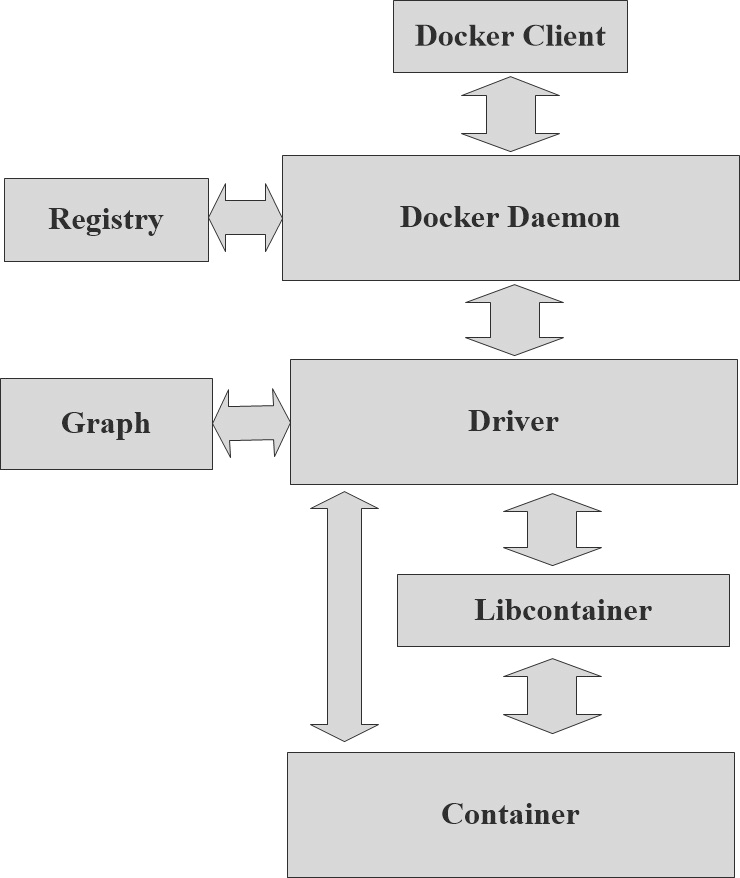
\includegraphics[width=1.0\textwidth]{Docker_Module}
    \caption{Docker运行模块结构图}
    \label{fig:docker_module}
\end{figure}

Docker使用了传统的Client-Server架构模式(C-S)。Docker Client为客户端,Docker Daemon为常驻后台的服务端。用户通过Unix Domain Socket(UDS)在Docker Client与Docker Daemon之间建立HTTP通信,用户对于docker的操作请求会被Docker Client翻译成HTTP通信指令,并发送到Docker Daemon,通过提供的API接口进行执行。Docker Daemon是Docker架构中的主体部分,是松耦合结构,包括Dockerfile编译、Registry镜像仓库通信、Graphdriver镜像管理驱动、Driver文件系统驱动、Libcontainer容器管理等模块,不同模块各司其职并有机组合,完成用户的请求。当用户需要下载镜像Image创建Docker容器时,首先,通过Docker Client向Docker Daemon发出命令请求,Docker Daemon解析后,会从远程Registry中下载镜像。随后,Docker通过Driver中的镜像管理驱动Graphdriver将下载的镜像以Graph的形式存储在本地。接下来,镜像管理驱动Graphdriver从Graph本地镜像存储目录中获取指定的镜像,并按照指定的规则为容器准备rootfs,rootfs以readonly方式加载并检查,然后在其上挂载writeable 层形成一个容器的运行目录。常用的Docker镜像的文件结构图如图\ref{fig:docker_image}所示。

\begin{figure}[!htbp]
    \centering
    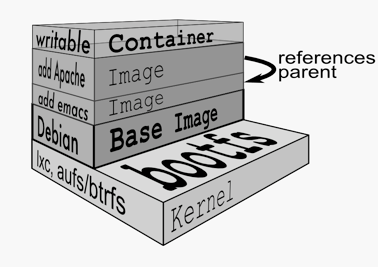
\includegraphics[width=1.0\textwidth]{Docker_Image}
    \caption{Docker运行模块结构图}
    \label{fig:docker_image}
\end{figure}

当需要为Docker容器创建网络环境时,则通过Driver中的网络管理驱动Libnetwork创建并配置Docker容器的网络环境;当需要限制Docker容器运行资源或执行用户指令等操作时,则通过Driver中的执行驱动Execdriver来完成。Libcontainer是一套实现容器管理的Go语言解决方案。这套解决方案实现过程中使用了Linux内核特性Namespace与Cgroups,同时还采用了Capability与文件权限控制等其他一系列技术。Libcontainer的设计初衷是希望该库可以不依靠任何依赖,直接访问内核中与容器相关的API。Docker可以直接调用Libcontainer,而最终操纵容器的Namespace、Cgroups、Apparmor、网络设备以及防火墙规则等,这一系列操作的完成都不需要依赖LXC或者其他包。基于这些特性,除了创建容器之外,Libcontainer还可以完成管理容器生命周期的任务。目前Libcontainer的目标是实现容器技术的统一API,即无论底层使用什么技术,只要实现了Libcontainer定义的一组接口,Docker都可以在上面运行。这也为Docker实现全面的跨平台带来了可能。为了实现这一目标,Libcontainer也逐渐从Docker Daemon中剥离出来,形成了Containerd。Containerd向Docker提供运行容器的API,二者通过grpc进行交互。Containerd最后会通过runc来实际运行容器。

% \subsection{容器集群技术}


% \section{自组织网络技术}
\section{计算迁移技术}\label{sec:related_work_computing_offloading}
\subsection{计算迁移技术}

传统的终端设备的服务模式通常是终端设备在本地进行计算任务的运行,依靠终端设备自身的计算能力来保证服务质量。而随着边缘智能终端设备所要承担的计算任务越来越重,终端设备资源受限问题使得单一终端设备本地计算难以满足终端服务和任务对终端计算能力的要求,计算迁移技术逐渐成为了一个可行的解决方案\cite{张文丽2016智能移动终端计算迁移研究}。计算迁移技术(Computation Offloading),也被称为计算卸载技术,是指将终端设备上的计算任务,通过网络的形式发送到其他设备上进行计算,再将计算结果通过网络返回给终端设备。计算迁移技术的目的是扩展终端设备的计算能力,为用户提供质量更好的终端服务。

经过十几年的发展,计算迁移技术逐渐成为云计算和边缘计算中的一项重要技术\cite{崔勇2017移动云计算研究进展与趋势}。通常使用的方法是将边缘终端设备上的计算任务根据具体需求迁移一部分或迁移全部到云端计算资源上进行处理,利用一部分通信开销来置换一部分计算、存储等资源,为用户提供质量更好的服务\cite{徐乃凡2018面向边缘云高效能的移动终端计算迁移方法}。云端计算资源通常是部署在云数据中心的机房,可以提供计算、存储、网络等资源,这种计算模式又被称为Mobile Cloud Computing (MCC)\cite{barbarossa2014communicating}。但是终端设备与云数据中心之间会出现大量数据交互,产生大量网络延迟,并且可能会出现信息泄露等隐患,终端服务的实时性与安全性都不能得到保证\cite{shi2016edge}。

为了拉近云数据中心与用户终端之间的距离,云端计算资源也会部署在网络边缘,例如基站、边缘服务器等等。这种计算模式又被称为Mobile Edge Computing (MEC)\cite{董浩2019移动边缘计算环境下服务工作流的计算卸载,mach2017mobile}。与MCC类似,MEC也是一种集中式的云计算资源,需要资源服务器、中央管理器、移动网络等基础设施的支持,部署起来会比较复杂。目前对于MEC中计算迁移技术的的研究,主要集中在计算迁移决策、计算资源管理及移动性管理三个方面,而对与MEC系统中的计算迁移方案的设计与实现研究较少\cite{谢人超2018移动边缘计算卸载技术综述}。

文献\cite{satyanarayanan2009case}中介绍了一种计算迁移系统,利用部署在用户身边的可信的、能连接网络的、计算资源丰富的计算设备或计算机集群(被称为cloudlet)为移动用户提供服务。当用户在终端设备上产生服务请求时,终端设备可以在cloudlet上快速建立定制化的虚拟机,将计算任务迁移到对应虚拟机中并利用其资源来运行,用户可以利用轻量级客户端通过无线网络进行访问\cite{verbelen2012cloudlets}。cloudlet模式是一种粗粒度的计算迁移技术\cite{谢人超2018移动边缘计算卸载技术综述}。cloudlet的实现过程需要迁移整个VM Overlay,迁移时间较长,需要60-90s,当终端附近的cloudlet资源不足以支撑起计算迁移服务的时候,终端会向远程的云端资源请求协助\cite{张文丽2016智能移动终端计算迁移研究}。cloudlet计算迁移模式相比MCC和MEC,与用户之间的距离更近,传输时延更小,非常适合图书馆、咖啡厅、办公室等聚集场所。但cloudlet的缺点是需要在区域内单独进行部署,需要额外的硬件、场地、服务器等成本,使用范围有局限性\cite{li2014can,zhang2018hybrid}。另外,对于cloudlet的计算迁移技术的研究也还存在着缺乏统一的部署和管理方法的不足\cite{张文丽2016智能移动终端计算迁移研究}。
\subsection{基于Web的计算迁移技术}
Web Worker是一种基于HTML5的多线程方法,本文的研究对象就是面向Web Worker的计算迁移系统。基于Web Worker的服务系统可以拥有更好的跨平台性,应用开发者在开发服务应用的过程中可以不必考虑底层的系统架构\cite{王硕2016嵌入式}。基于Web Worker的计算迁移方法分为透明迁移和非透明迁移两类\cite{wang2018html5}。基于Web Worker的非透明迁移通常采用的方法是重写标准的Web Worker的接口API,并在编写Web应用的时候以新的库的形式导入修改,使得Web应用在运行的时候通过WebSocket通知运行在云端的服务端程序生成相应的Web Worker来进行计算\cite{zbierski2014bring,hwang2014wwf,hwang2014cloud,gong2016wwof,kurumatani2012executing}。文献\cite{王昭2018Web}中提出了一种基于Web Worker的非透明迁移方法,通过重写Web应用的库,将终端上HTML的Web Worker迁移到其他服务器或其他终端设备上进行计算。文献\cite{zhang2010elastic}中提出了一种基于Web Worker的透明迁移方法,通过修改Web Worker运行环境代码来实现计算迁移的过程,但是没有做具体实现。

\section{任务调度算法}\label{sec:related_work_task_scheduling}
任务调度问题是一种在云计算\cite{qiao2016efficient}、边缘计算\cite{guo2017energy}、海服务\cite{王劲林2015一种现场}等领域常见的问题。在基于容器化的多终端协同服务技术种,不同的终端所能够提供的资源类型和大小不同,不同的任务对于不同类型资源的消耗情况也不一样,当然不同任务在不同节点上执行的费用和时间也不同。智能终端的资源是受限的,合理规划任务在节点上的执行调度,能够减少资源碎片,提高终端资源利用率\cite{huang2013energy,tseng2014effective,马晓光2017一种适用于}。任务调度问题是一种NP-hard问题\cite{tawfeek2013cloud},难以通过计算得到精确的数值最优解,需要通过将任务调度问题划归为一类优化问题(Optimization Problem),建立寻优的数学模型,利用一些寻优算法来获得一个近似最优解。常用的解决方法是传统的基于贪心策略的任务调度优化算法,以及元启发式优化算法。

\subsection{传统任务调度算法}

有很多传统的基于贪心策略的任务调度优化算法\cite{乔楠楠2017一种面向网络边缘任务调度问题的多方向粒子群优化算法}。先进先出算法(FIFO Scheduler)是按照任务到达的先后顺序进行调度\cite{zaharia2009job},Max-Min算法是优先调度执行时间最长的任务,Min-Min算法是优先调度执行时间最短的任务,\cite{tabak2014improving,杜玉霞2010Min}。这些基于贪心策略的任务调度算法的优点是原理比较简单,方便实施,运行速度快。由于这些算法的原理过于简单,优先满足局部最优选择,导致其缺点是很容易陷入局部最优解,得不到效果更好的解决方案。尤其是当任务规模扩大的时候,任务的维度也会增加,这会扩大搜索空间并使优化问题更加复杂,基于贪心策略的传统任务调度算法无法处理这种情况。

\subsection{元启发式算法}

近年来,很多元启发式算法(meta-heuristic algorithm)被应用于解决任务调度问题\cite{al2015cloudlet,刘运2015基于高斯变异的人工萤火虫算法在云计算资源调度中的研究}。Goldberg在1988年提出的遗传算法(Genetic Algorithm,GA)是一种非常著名的进化算法,它将自然选择理论引入到优化过程中,使用一条染色体来代表任务调度问题的一种调度方案,使用包括变异、交叉和选择在内的几个自然算子来作为演进迭代的计算法则\cite{fonseca1995overview,whitley1994genetic}。由于存在交叉和变异的操作,GA计算起来非常复杂,实现起来也比较困难。

一些元启发式算法的灵感来自昆虫,鱼类,鸟类和其他群体生物的自然行为。粒子群算法(Particle Swarm Optimization Algorithm,PSO)是Kennedy于1995年提出的经典元启发式算法,原理非常简单,容易实现\cite{kennedy1995particle,liao2007discrete,krishnasamy2013task}。蚁群优化算法(Ant Colony Optimization Algorithm,ACO)的灵感来自蚂蚁在巢穴和食物来源之间搜索的自然觅食行为,蚁群优化算法利用化学信息素在蚁群搜索单位之间进行信息交流\cite{dorigo1997ant,dorigo1999ant,Hao2018Network}。人工鱼群算法通过模仿鱼类的随机游动的觅食行为来进行搜索\cite{桓自强2014aafsa}。

近年来,一些较新的元启发式算法也被提出,而且以这些元启发式算法为基础的改进并不多。2015年提出的蚁狮算法(Ant Lion Optimizer,ALO)的灵感来自于蚁群的狩猎行为\cite{mirjalili2015ant}。鲸鱼优化算法(Whale Optimization Algorithm,WOA)于2016年提出,该算法模拟鲸鱼的自然狩猎行为\cite{mirjalili2016whale}。2016年提出的蜻蜓算法(Dragonfly Algorithm,DA)基于自然界中蜻蜓群的静态和动态行为进行搜索\cite{mirjalili2016dragonfly}。2017年,Shahrzad Saremi和Seyedali Mirjalili提出了一种名为蝗虫优化算法(Grasshopper Optimization Algorithm,GOA)的新型元启发式优化算法。 蝗虫优化算法利用群体内相互作用力的影响和群体外的风力及食物来源修正的影响来模拟蝗虫群的迁移及觅食行为,以求寻找到目标食物\cite{saremi2017grasshopper}。蝗虫优化算法利用群体智慧,通过共享蝗虫群体的经验来确定搜索方向并找到最佳或近似最佳位置。蝗虫优化算法还使用演进的方法进行多次迭代,以使群体智慧更加有效。
% \section{预测算法}

\section{本章小结}\label{sec:related_work_summary}

本章主要介绍了本文研究所涉及到的相关技术的概念以及研究现状。本章首先介绍了云计算技术与边缘计算技术的概念与特点;其次介绍了虚拟化技术的起源与发展现状;然后介绍了计算迁移技术的研究现状及几种计算迁移方案的特点;最后介绍了任务调度问题和解决方法,尤其是几种近几年新提出的元启发式优化算法。本章相关技术的介绍,成为本文后续几章研究工作的基础。